% This is samplepaper.tex, a sample chapter demonstrating the
% LLNCS macro package for Springer Computer Science proceedings;
% Version 2.20 of 2017/10/04
%
\documentclass[runningheads]{llncs}
%
\usepackage{graphicx}
% Used for displaying a sample figure. If possible, figure files should
% be included in EPS format.
%
% If you use the hyperref package, please uncomment the following line
% to display URLs in blue roman font according to Springer's eBook style:
% \renewcommand\UrlFont{\color{blue}\rmfamily}

\begin{document}
%
\title{Daily Readiness Score Prediction}
%
%\titlerunning{Abbreviated paper title}
%If the paper title is too long for the running head, you can set
%an abbreviated paper title here

\author{Daria Potoskueva (1871845)
%\inst{1}\orcidID{0000-1111-2222-3333} 
\and Ki duk Kang (1871730)
%\inst{2,3}\orcidID{1111-2222-3333-4444} 
\and
Ignatius Jordi Bernandi Harsawiguna (1871833)
\and
Shiyu Li (1869814)
\and
Yi Wang (1870245)
\and
Yiyi Wei (1873027)}
%\inst{3}\orcidID{2222--3333-4444-5555}}
%
\authorrunning{F. Author et al.}
% First names are abbreviated in the running head.
% If there are more than two authors, 'et al.' is used.
%
\institute{Princeton University, Princeton NJ 08544, USA \and
Springer Heidelberg, Tiergartenstr. 17, 69121 Heidelberg, Germany
\email{lncs@springer.com}\\
\url{http://www.springer.com/gp/computer-science/lncs} \and
ABC Institute, Rupert-Karls-University Heidelberg, Heidelberg, Germany\\
\email{\{abc,lncs\}@uni-heidelberg.de}}
%
\maketitle              % typeset the header of the contribution
%
\begin{abstract}
The abstract should briefly summarize the contents of the paper in
15--250 words.

\keywords{First keyword  \and Second keyword \and Another keyword.}
\end{abstract}
%
%
%
\section{Application area and goals}
Nowadays many people cannot imagine their lives without digital technologies. This kind of technology allows people to store their data which are related not only to their leisure time, but also to their health. The information about people's condition is stored by different gadgets or/and applications. This kind of data is used for maintaining people's health by aforementioned technologies. Moreover, these days people prefer caring about their health by doing sports. In order to control their condition daily or/and during trains people  wear smartwatches. These devices not only store data, but also are able to predict some of them for a future day/days. Based on data from such devices, we would like to predict people's readiness to work out for upcoming day. This characteristic is of great importance for people, since in most cases they assess their readiness for sports based on their current feelings which are connected with previous days condition. The goal of this project is to find out the best classification model for prediction readiness of a person based on data for preceding days. We have decided to explore classification approaches due to the fact that attribute "readiness" in using data is assessed in the range 0 - 10, where 0 is assigned to a person whom isn't ready to do sports for upcoming day and 10 is assigned to a person whom is ready for extra work out for upcoming day.


\section{Profile of a data set}
The explored data set consists of traditional lifelogging data and sports activity logging data which has been collected by using Fitbit Versa 2 smartwatch wristband, the PMSys sports logging application, and forms in Google. The data has been gathered within 5 months (from November 2019 to March 2020) and contains information about 16 people on the age scale 25 - 60 years and with a mean value of the age of 34 years. Furthermore, during the collection of the data, the participants have been advised to do exercises at least twice per week (without any particular restrictions on exercises or their duration). The range of people's experience in sports is from participants who do exercises rare to active athletes.

The structure of explored data set is placed below in Figure 1. Moreover, parts from different resources are highlighted with various colors which depend on the place where the data has been stored:

\begin{figure}[h]
\centerline{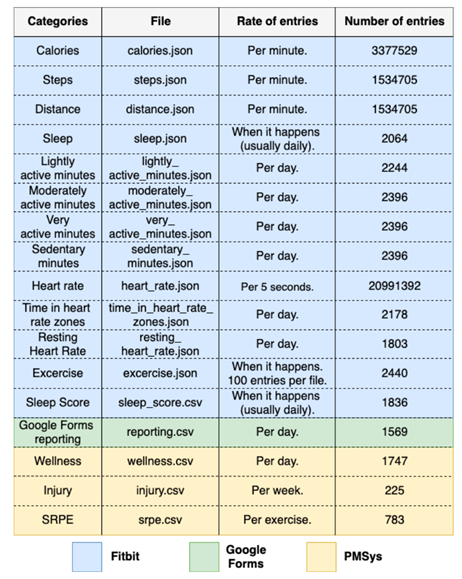
\includegraphics{structure.png}}
\caption{An overview of explored data set.\orcidID{1}}
\label{fig}
\end{figure}

The following data has been collected by using the Fitbit Versa 2:
\begin{itemize}
    \item calories - shows the digit of calories which the participant has burned per minute;
    \item steps - shows the digit of steps which has been passed per minute;
    \item distance - shows the distance which has been passed per minute in cm;
    \item sleep - shows the splitting of sleep zones into light, deep and rapid, also, shows the waking time in minutes;
    \item lightly active minutes - shows the amount of slightly active minutes for a day;
    \item moderately active minutes - shows the digit of minutes spent in moderate activity for a day;
    \item very active minutes - shows the digit of minutes spent actively for a day;
    \item sedentary minutes - shows the digit of minutes spent in a sitting position for a day;
    \item heart rate - shows the digit of heartbeats for a minute for the estimated time;
    \item time in heart rate zones - shows the digit of minutes in the following heart rate zones: fat burn (from 50 to 69\% of a person's maximum heart rate), cardio (from 70 to 84\% of a person's maximum heart rate), peak (from 85 to 100\% of a person's maximum heart rate), where the person's maximum heart rate is calculated as 220 minus the participant's age;
    \item resting heart rate - the value which shows daily resting heart rate;
    \item exercise - shows the information which is related to a specific activity such as the date, activity duration, kind of activity, etc.;
    \item sleep score - assigned score (from 0 to 100) for each night's sleep. Each score is calculated based on indicators of composition, recovery, and duration, the digit of minutes of deep sleep, resting heart rate, and anxiety score.
\end{itemize}

The following data has been collected by using forms in Google:
\begin{itemize}
    \item google forms reporting - consists of subjective reporting data for a day, which contain the date and time of a report, meals, the weight of a participant, the digit of glasses drunk, and alcohol consumption.
\end{itemize}

The rest of data has been collected by using the PMSys sports logging application:
\begin{itemize}
    \item wellness - consists of information about date and time, tiredness (has a range of score from 1 to 5, where 3 is a normal score, 1 or 2 is below normal one and 4 or 5 is above), mood of a participant (has the same range as tiredness), readiness (measure whether a participant is ready to work out this day or not; has a range of score from 0 to 10, where 0 means that the participant isn't ready at all and 10 that the person is ready for an extra work out), number of hours of sleep, the quality of sleep (has the same range as tiredness), soreness (has the same range as tiredness) and its area, stress (has the same range as tiredness);
    \item injury - indicates whether a participant has injuries, also contains date and time, the location of the injury, the information on how bad it is;
    \item srpe - shows the end-time of a train, kind of activity, sensed exertion, the number of minutes for a training session.
\end{itemize}

\section{Preprocessing and Mining}

%\subsection{A Subsection Sample}
%Please note that the first paragraph of a section or subsection is
%not indented. The first paragraph that follows a table, figure,
%equation etc. does not need an indent, either.

%Subsequent paragraphs, however, are indented.

%\subsubsection{Sample Heading (Third Level)} Only two levels of
%headings should be numbered. Lower level headings remain unnumbered;
%they are formatted as run-in headings.

\paragraph{Sample Heading (Fourth Level)}
The contribution should contain no more than four levels of
headings. Table~\ref{tab1} gives a summary of all heading levels.

\begin{table}
\caption{Table captions should be placed above the
tables.}\label{tab1}
\begin{tabular}{|l|l|l|}
\hline
Heading level &  Example & Font size and style\\
\hline
Title (centered) &  {\Large\bfseries Lecture Notes} & 14 point, bold\\
1st-level heading &  {\large\bfseries 1 Introduction} & 12 point, bold\\
2nd-level heading & {\bfseries 2.1 Printing Area} & 10 point, bold\\
3rd-level heading & {\bfseries Run-in Heading in Bold.} Text follows & 10 point, bold\\
4th-level heading & {\itshape Lowest Level Heading.} Text follows & 10 point, italic\\
\hline
\end{tabular}
\end{table}


\noindent Displayed equations are centered and set on a separate
line.
\begin{equation}
x + y = z
\end{equation}
Please try to avoid rasterized images for line-art diagrams and
schemas. Whenever possible, use vector graphics instead (see
Fig.~\ref{fig1}).

\begin{figure}
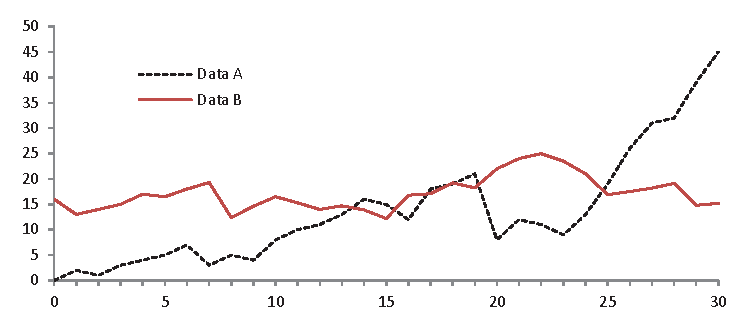
\includegraphics[width=\textwidth]{fig1.eps}
\caption{A figure caption is always placed below the illustration.
Please note that short captions are centered, while long ones are
justified by the macro package automatically.} \label{fig1}
\end{figure}

\begin{theorem}
This is a sample theorem. The run-in heading is set in bold, while
the following text appears in italics. Definitions, lemmas,
propositions, and corollaries are styled the same way.
\end{theorem}
%
% the environments 'definition', 'lemma', 'proposition', 'corollary',
% 'remark', and 'example' are defined in the LLNCS documentclass as well.
%
\begin{proof}
Proofs, examples, and remarks have the initial word in italics,
while the following text appears in normal font.
\end{proof}
For citations of references, we prefer the use of square brackets
and consecutive numbers. Citations using labels or the author/year
convention are also acceptable. The following bibliography provides
a sample reference list with entries for journal
articles~\cite{ref_article1}, an LNCS chapter~\cite{ref_lncs1}, a
book~\cite{ref_book1}, proceedings without editors~\cite{ref_proc1},
and a homepage~\cite{ref_url1}. Multiple citations are grouped
\cite{ref_article1,ref_lncs1,ref_book1},
\cite{ref_article1,ref_book1,ref_proc1,ref_url1}.
%
% ---- Bibliography ----
%
% BibTeX users should specify bibliography style 'splncs04'.
% References will then be sorted and formatted in the correct style.
%
% \bibliographystyle{splncs04}
% \bibliography{mybibliography}
%
\begin{thebibliography}{8}
\bibitem{ref_article1}
Author, F.: Article title. Journal \textbf{2}(5), 99--110 (2016)

\bibitem{ref_lncs1}
Author, F., Author, S.: Title of a proceedings paper. In: Editor,
F., Editor, S. (eds.) CONFERENCE 2016, LNCS, vol. 9999, pp. 1--13.
Springer, Heidelberg (2016). \doi{10.10007/1234567890}

\bibitem{ref_book1}
Author, F., Author, S., Author, T.: Book title. 2nd edn. Publisher,
Location (1999)

\bibitem{ref_proc1}
Author, A.-B.: Contribution title. In: 9th International Proceedings
on Proceedings, pp. 1--2. Publisher, Location (2010)

\bibitem{ref_url1}
LNCS Homepage, \url{http://www.springer.com/lncs}. Last accessed 4
Oct 2017
\end{thebibliography}
\end{document}
